% 2011 年四川卷理科第 21 题：椭圆 x^2+y^2/2=1，顶点 A(-1,0)、B(1,0)，焦点 F(0,1)，
%   过 F 的直线 l 交椭圆于 C、D，交 x 轴于 P，直线 AC 与 BD 交于 Q。
% 来源 PDF：普通高考/2011/2011四川理.pdf，SHA-256 116ce515679869425079ef4777505df3735ba4cba64847c9069b7d7acdb4fda4。
% 原页：第 2 页（A3 三栏）第 2 栏中部，书页码 702。
% 重绘依据：照原页——椭圆竖长（半轴 1 与 √2），A 为左顶点、B 为右顶点，F 在 O 上方；
%   l 自左上（过 D）经 F、C 交 x 轴于 B 右侧的 P，并越过 P 继续向右下；
%   AC 自 A 过 C 向右上延长，BD 自 B 过 D 向左上延长，二者交于 Q（椭圆内、O 右侧）。
%   取 l 的斜率 k=-0.55，各点按解析式算得，不按原页比例。
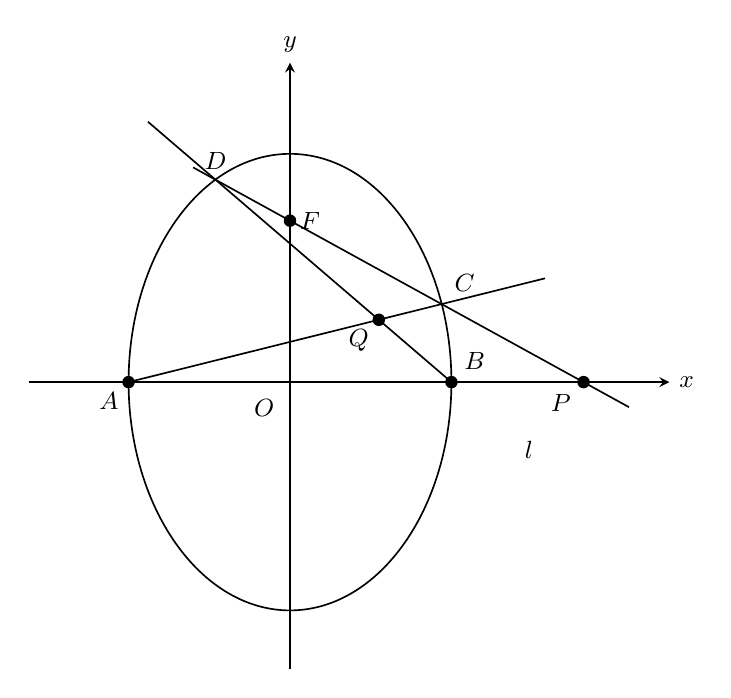
\begin{tikzpicture}[scale=2.05, >=stealth, semithick, font=\small]
  % 坐标轴
  \draw[->] (-1.62,0) -- (2.35,0) node[right] {$x$};
  \draw[->] (0,-1.78) -- (0,1.98) node[above] {$y$};

  % 椭圆
  \draw (0,0) ellipse (1 and 1.41421);

  % 各点
  \coordinate (A) at (-1,0);
  \coordinate (B) at (1,0);
  \coordinate (F) at (0,1);
  \coordinate (C) at (0.9397,0.4832);
  \coordinate (D) at (-0.4619,1.2540);
  \coordinate (P) at (1.8182,0);
  \coordinate (Q) at (0.55,0.3861);

  % 直线 l
  \draw (-0.60,1.330) -- (2.10,-0.155);
  % 直线 AC、BD 及其延长
  \draw (A) -- (1.58,0.643);
  \draw (B) -- (-0.88,1.613);

  \fill (A) circle (1.1pt);
  \fill (B) circle (1.1pt);
  \fill (F) circle (1.1pt);
  \fill (P) circle (1.1pt);
  \fill (Q) circle (1.1pt);

  \node at (A) [below left] {$A$};
  \node at (B) [above right=1pt] {$B$};
  \node at (F) [right] {$F$};
  \node at (C) [above right=1pt] {$C$};
  \node at (D) [above] {$D$};
  \node at (P) [below left=1pt] {$P$};
  \node at (Q) [below left] {$Q$};
  \node at (-0.16,-0.16) {$O$};
  \node at (1.48,-0.42) {$l$};
\end{tikzpicture}
